\chapter{绪论}

随着互联网的不断发展,以及终端设备,比如手机,拍照设备,监控设备的广泛应用,互联网上现在保存的图片数量巨大,并且每天都在以惊人的速度增长,有数据显示,2011年FaceBook上就存储了多达1000亿张图片,并且每天以3已张的速度在增长。如何在巨大的图像库中精确并且快速的找到相应的图片,逐渐成为研究的热点。该问题是大数据处理及图像处理两个计算机领域问题的交叉。大数据处理技术在近年来无疑是最受关注的研究问题之一,其他的还有云计算及人工智能,三者有着紧密的联系。基于内容的图像检索在大数据下的图像检索背景下受到研究者们的重视,该技术充分利用图片自身的信息,不需要人工的为每张图片打上描述标签,较传统的以标签搜图技术,有极大的匹配精度。现在百度和google公司都有相应的以图搜图服务,用户通过上传相似图片,搜索系统将返回匹配成功的相似结果。

\section{研究背景}
本小节先介绍图像检索的基本概念,然后引出以图搜图的存在意义,再从以图搜图引出图像特征提取及大数据处理等关键技术。

\subsection{图像检索}
早在20世纪70年代,就出现了关于图像检索技术的研究,当时主要是基于文本的图像检索(Text-based Image Retrieval)技术,利用文本描述的方式描述图像的特征,比如图像的名称,图像的尺寸,压缩的类型,作者,然后以关键词的形式提问查询图像,或者是根据等级目录的形式浏览查找特定目录下的图像,如Getty AAT使用近133,000个术语来描述艺术、艺术史、建筑以及其它文化方面的对象,并推出30多个等级目录,从7方面描述图像的概念、物理属性、类型和刊号等。又如Gograph)将图像分为动态图像、照片、图标、背景、艺术剪辑图、插图、壁纸、界面、成套图像8个一级类,下设数量不等的子类。在图像数字化之前,档案管理者、图书管理员都是采用这种方式组织和管理图像。 图像所在页面的主题、图像的文件名称、与图像密切环绕的文字内容、图像的链接地址等都被用作图像分析的依据,根据这些文本分析结果推断其中图像的特征。

基于文本的检索技术发展已经十分成熟了,比如Page-Rank方法、概率方法、位置方法、摘要方法、分类或聚类方法、词性标注法等都已十分成熟的应用于文本检索中,并且基于文本的图像检索分析和实现难度略小。但是因为受控词汇本身的局限,易歧义,更新慢,所以不太容易应对网络上日新月异的各类图像。为了更加准确的表达搜索的意图,更加精确的搜索目标图像,基于内容的图像检索(Content-based Image Retrieval)技术逐渐发展起来。

基于内容的图像检索技术是利用图像的颜色,纹理,布局等信息进行分析和检索的图像技术,因为检索的线索十分明确,因此查找的精确度十分高,但是上述的这些信息是要远大文本信息的,在检索速度和效率上要求更高。目前已有不少的应用于实际环境的CBIR图像检索系统,比如IBM公司开发的最早商业化的QBIC系统,以及由哥伦比亚大学研发的WebSeek系统、麻省理工学院研发的Photobook系统,百度及谷歌公司的以图搜图搜索服务等,以图搜图的常见框架如下图所示:
\begin{figure}[htp]
\centering
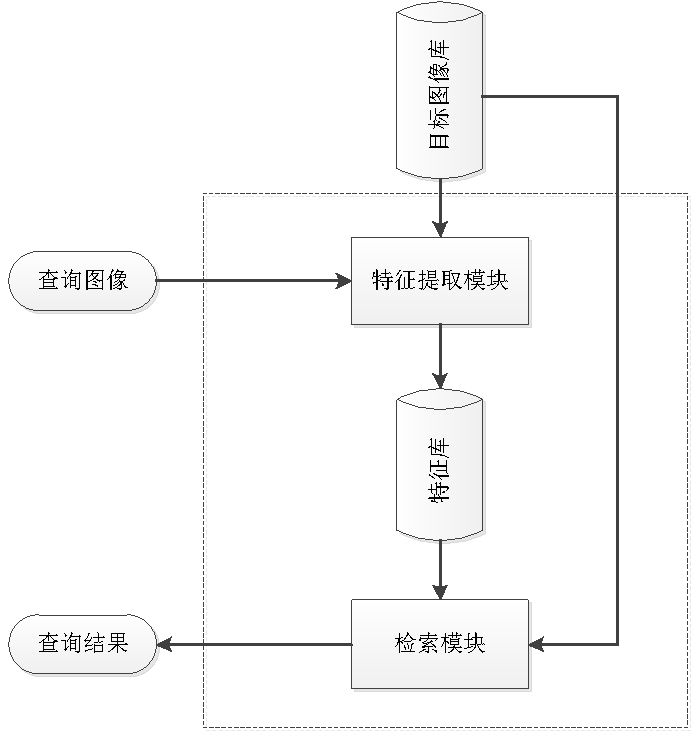
\includegraphics{retrivelfw}
\caption{基于内容的图像检索框架}
\end{figure}
\\先将检索系统的图像库通过特征提取模块进行特征提取,将提取出来的特征保存到系统的特征库中,查询图像先通过特征提取模块进行特征提取,然后检索模块通过匹配查询图片的特征和特征库存在的特征,最后返回匹配的结果。

上面运行步骤中,主要涉及两个图像处理的中关键技术,分别是特征提取和特征匹配。特征提取最为重要,因为如果特征提取做的不好,会直接影响后面的所有步骤,因此如果快速并且提取高质量的图像特征,一直是研究的热点。

\subsection{特征提取}
因为在计算机中,处理的只有数字信号,为了使计算机能够”理解“图像,我们必须从图像中提取有用的信息,得到图像的”非图像“表示或描述,比如数值,向量或者是符号,这一过程就是图像的特征提取。
\subsubsection{特征分类}
至今为止,对于图像特征没有万能和精确的定义,对特征的定义往往由问题或者应用的类型决定的。图像特征大体可以分为两类,分别是全局特征和局部特征。常见关注的图像全局特征有颜色特征,纹理特征,形状特征,空间关系特征等;局部特征则有斑点,角点,边缘以及脊等。因为局部特征只反映图像上的局部特殊性,往往对应着图像中的一些线条交叉,明暗变化结构,受到噪声的干扰比较少,所以适合做图像的匹配和检索操作;全局特征关注的是全局的特性,比如颜色分布,纹理特征,物体形状等,全局特征适合对图像的理解,但是由于容易受到光照,旋转,噪声的影响,不适合进行图像的匹配和检索工作。常见的全局特征及局部特征描述如下:
\begin{itemize}
\item 颜色特征\\颜色特征是一种全局特征,描述了图像或图像区域所对应的景物的表面性质。一般颜色特征是基于像素点的特征,此时所有属于图像或图像区域的像素都有各自的贡献。由于颜色对图像或图像区域的方向、大小等变化不敏感,所以颜色特征不能很好地捕捉图像中对象的局部特征。另外,仅使用颜色特征查询时,如果数据库很大,常会将许多不需要的图像也检索出来。颜色直方图是最常用的表达颜色特征的方法,其优点是不受图像旋转和平移变化的影响,进一步借助归一化还可不受图像尺度变化的影响,基缺点是没有表达出颜色空间分布的信息。
\item 纹理特征\\纹理特征也是一种全局特征,它也描述了图像或图像区域所对应景物的表面性质。但由于纹理只是一种物体表面的特性,并不能完全反映出物体的本质属性,所以仅仅利用纹理特征是无法获得高层次图像内容的。与颜色特征不同,纹理特征不是基于像素点的特征,它需要在包含多个像素点的区域中进行统计计算。在模式匹配中,这种区域性的特征具有较大的优越性,不会由于局部的偏差而无法匹配成功。作为一种统计特征,纹理特征常具有旋转不变性,并且对于噪声有较强的抵抗能力。但是,纹理特征也有其缺点,一个很明显的缺点是当图像的分辨率变化的时候,所计算出来的纹理可能会有较大偏差。另外,由于有可能受到光照、反射情况的影响,从2-D图像中反映出来的纹理不一定是3-D物体表面真实的纹理。
\item 形状特征\\各种基于形状特征的检索方法都可以比较有效地利用图像中感兴趣的目标来进行检索,但它们也有一些共同的问题,包括:1)目前基于形状的检索方法还缺乏比较完善的数学模型;2)如果目标有变形时检索结果往往不太可靠;3)许多形状特征仅描述了目标局部的性质,要全面描述目标常对计算时间和存储量有较高的要求;4)许多形状特征所反映的目标形状信息与人的直观感觉不完全一致,或者说,特征空间的相似性与人视觉系统感受到的相似性有差别。另外,从 2-D 图像中表现的 3-D 物体实际上只是物体在空间某一平面的投影,从 2-D 图像中反映出来的形状常不是 3-D 物体真实的形状,由于视点的变化,可能会产生各种失真。
\item 空间关系特征\\所谓空间关系,是指图像中分割出来的多个目标之间的相互的空间位置或相对方向关系,这些关系也可分为连接/邻接关系、交叠/重叠关系和包含/包容关系等。通常空间位置信息可以分为两类:相对空间位置信息和绝对空间位置信息。前一种关系强调的是目标之间的相对情况,如上下左右关系等,后一种关系强调的是目标之间的距离大小以及方位。显而易见,由绝对空间位置可推出相对空间位置,但表达相对空间位置信息常比较简单。空间关系特征的使用可加强对图像内容的描述区分能力,但空间关系特征常对图像或目标的旋转、反转、尺度变化等比较敏感。另外,实际应用中,仅仅利用空间信息往往是不够的,不能有效准确地表达场景信息。为了检索,除使用空间关系特征外,还需要其它特征来配合。
\item 角点 \\角点经常被检测在边缘的交界处、被遮挡的边缘、纹理性很强的部分。
\item 斑点\\斑点通常是指与周围有着颜色和灰度差别的区域,如草原上的一棵树或一栋房子。由于斑点代表的是一个区域,相比单纯的角点,它的稳定性要好,抗噪声能力要强,所以它在图像配准上扮演了很重要的角色。
\item 边缘 \\边缘是组成两个图像区域之间边界(或边缘)的像素。一般一个边缘的形状可以是任意的,还可能包括交叉点。在实践中边缘一般被定义为图像中拥有大的梯度的点组成的子集。一些常用的算法还会把梯度高的点联系起来来构成一个更完善的边缘的描写。这些算法也可能对边缘提出一些限制。
\item 脊 \\长条形的物体被称为脊。在实践中脊可以被看作是代表对称轴的一维曲线,此外局部针对于每个脊像素有一个脊宽度。从灰梯度图像中提取脊要比提取边缘、角和区域困难。在空中摄影中往往使用脊检测来分辨道路,在医学图像中它被用来分辨血管。
\end{itemize}
\subsubsection{提取算法}
不同类型的特征对应着不同的提取算法,算法的原理不一样,提取精度不一样,计算复杂性也不一样。
\begin{itemize}
\item 颜色直方图法\\它能简单描述一幅图像中颜色的全局分布,即不同色彩在整幅图像中所占的比例,特别适用于描述那些难以自动分割的图像和不需要考虑物体空间位置的图像。其缺点在于:它无法描述图像中颜色的局部分布及每种色彩所处的空间位置,即无法描述图像中的某一具体的对象或物体。
\item 颜色集 \\颜色直方图法是一种全局颜色特征提取与匹配方法,无法区分局部颜色信息。颜色集是对颜色直方图的一种近似首先将图像从 RGB颜色空间转化成视觉均衡的颜色空间(如 HSV 空间),并将颜色空间量化成若干个柄。然后,用色彩自动分割技术将图像分为若干区域,每个区域用量化颜色空间的某个颜色分量来索引,从而将图像表达为一个二进制的颜色索引集。
\item 灰度共生矩阵\\ 该方法是一种具有统计意义的纹理特征分析方法。Gotlieb 和 Kreyszig 等人在研究共生矩阵中各种统计特征基础上,通过实验,得出灰度共生矩阵的四个关键特征:能量、惯量、熵和相关性。
\item 几何法\\几何法是是建立在纹理基元(基本的纹理元素)理论基础上的一种纹理特征分析方法。纹理基元理论认为,复杂的纹理可以由若干简单的纹理基元以一定的有规律的形式重复排列构成。在几何法中,比较有影响的算法有两种:Voronio 棋盘格特征法和结构法。
\item 边界特征法\\该方法通过对边界特征的描述来获取图像的形状参数。其中Hough 变换检测平行直线方法和边界方向直方图方法是经典方法。Hough 变换是利用图像全局特性而将边缘像素连接起来组成区域封闭边界的一种方法,其基本思想是点—线的对偶性;边界方向直方图法首先微分图像求得图像边缘,然后,做出关于边缘大小和方向的直方图,通常的方法是构造图像灰度梯度方向矩阵。
\item 傅里叶形状描述符法\\傅里叶形状描述符(Fourier shape deors)基本思想是用物体边界的傅里叶变换作为形状描述,利用区域边界的封闭性和周期性,将二维问题转化为一维问题。
\item 尺度不变特征转换法\\尺度不变特征转换(Scale-invariant feature transform或SIFT)是一种电脑视觉的算法用来侦测与描述影像中的局部性特征,它在空间尺度中寻找极值点,并提取出其位置、尺度、旋转不变量。它是一种基于斑点检测的局部特征提取算法,对于光线、噪声、些微视角改变的容忍度相当高,在母数庞大的特征数据库中,很容易辨识物体而且鲜有误认。
\item Harris角点检测法\\该算法提出了应用邻近像素点灰度差值概念,利用移动的窗口在图像中计算灰度变化值,其中关键流程包括转化为灰度图像、计算差分图像、高斯平滑、计算局部极值、确认角点。
\end{itemize}

本文是以SIFT算法作为研究点,将其应用于大数据处理框架上,完成大规模图像库的快速提取工作,本文将在第二章详细介绍SIFT算法的原理。

\subsection{特征匹配}
除了特征提取之外,特征匹配也是图像处理中十分重要的技术。对于基于内容的图像检索,其匹配实际就是相似搜索或者是近似搜索问题。相似搜索是指对于给定的查询数据对象,在目标对象集合中找到和查询对象相似的对象。匹配的关键在于相似度的定义,常见的相似度的度量方式有下面几种:
\begin{itemize}
\item 汉明距离。对于两个长度为d的二进制字符串x和y,它们之间的距离使用汉明距离来度量,其定义如下:
\begin{equation}\label{hanming}
Ha=\sum_{1}^d(x_i=y_j)
\end{equation}

\item $l_p$ 范数距离。对于d维实数空间$R_d$中的两个向量点x=($x_1$,...,$x_d$)和y=($y_1$,...,$y_d$),x和y之间$l_p$-范数距离定义为:
\begin{equation}\label{fanshu}
L_p(x_i,y_i)=\Bigl(\sum_{l=1}^n(x_i-y_i)^p\Bigr)^\frac{1}{p}
\end{equation}

\item 余弦距离。设x和y为对于d维实数空间$R_d$中两个非零向量,它们之间的余弦距离定义如下公式所示:
\begin{equation}\label{yuxian}
\cos(x,y)=\frac{xy}{|x|_2|y|_2}
\end{equation}

\item Jaccard距离。对于两个集合A和B,它们之间的Jaccard距离定义如下:
\begin{equation}\label{Jaccard}
Ja(A,B)=\frac{|{A}\cap{B}|}{|{A}\cup{B}|}
\end{equation}
\end{itemize}

特征向量的维度越高,特征的描述也越详细,匹配的精度也就越高,如常见的sift特征是128维,Gist特征是960维,深度学习提取的特征维度是1024维甚至更高。在面对着这些高维的特征向量时,如果完全单纯的计算每个向量间的距离,匹配速度将会十分缓慢,因此如何在保证精度的情况下,提升匹配的效率,是一个技术难点。面对高维特征向量,可以通过给特征建立有效的索引来提升查询效率,比如KD-tree,R-Tree或者SR-tree 等,这些方法将相似的数据划分到同一个区域,建立一个层次型的组织结构。建立索引方式在面对着超高维特征向量时,效率还是偏低,有学者提出了降维的思想,将超高维向量降低到某个维度,牺牲部分精度来大幅度提升查询效率,最著名的就是局部敏感哈希算法,该方法通过适当的调节参数,可以保证很高的精确度条件下也有很高的查询效率。该算法目前已经被广泛的应用于文本聚类,语言统计等领域。

特征匹配方法在本设计工作中只是充当验证特征提取正确性的角色,并不是研究的重点。

\subsection{大数据处理处理技术}
我们现在生活在一个信息量爆炸的时代,各行各业现在都面临着数据处理的压力,无论是处理的数据量,还是处理的速度,单台机器早已无法满足当今大数据应用的处理要求了,因此我们需要有一个大数据背景下的数据处理或者是存储框架,以帮助我们更加轻松的处理海量数据。在这种背景下,许多优秀的大数据处理框架逐渐诞生。接下来,本文将会介绍spark和HDFS两个大数据框架,它们都成功的应用于本文的设计工作中。
\subsubsection{内存计算框架spark}
Apache Spark 是专为大规模数据处理而设计的快速通用的计算引擎。Spark是UC Berkeley AMP lab (加州大学伯克利分校的AMP实验室)所开源的类Hadoop MapReduce的通用并行框架,Spark,拥有Hadoop MapReduce所具有的优点;但不同于MapReduce的是Job中间输出结果可以保存在内存中,从而不再需要读写HDFS,因此Spark能更好地适用于数据挖掘与机器学习等需要迭代的MapReduce的算法。Spark 是一种与 Hadoop 相似的开源集群计算环境,但是两者之间还存在一些不同之处,这些有用的不同之处使 Spark 在某些工作负载方面表现得更加优越,换句话说,Spark 启用了内存分布数据集,除了能够提供交互式查询外,它还可以优化迭代工作负载。

除了Map和Reduce操作之外,Spark还提供了丰富的生态应用环境,比如提供了SQL与结构化数据处理工具Spark SQL,机器学习工具MLib,分布式图计算引擎Graphx以及流式处理工具Spark Streaming。同时Spark的编程接口十分丰富,支持Scala,java,Python和R语言。Spark框架如图~\ref{fig:sparkfw}所示:
\begin{figure}[htp]
\centering
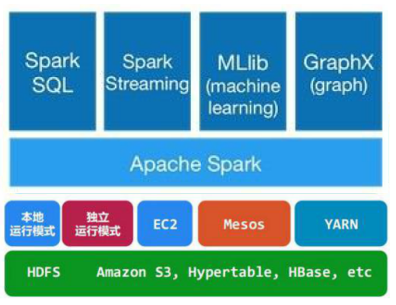
\includegraphics{sparkfw}
\caption{spark框架}
\label{fig:sparkfw}
\end{figure}

Spark的核心RDD(Resilient Distributed Datasets)[引用],是一个容错的、并行的数据结构,可以让用户显式地将数据存储到磁盘和内存中,并能控制数据的分区。同时,RDD还提供了一组丰富的操作来操作这些数据。在这些操作中,诸如map、flatMap、filter等转换操作实现了monad模式,很好地契合了Scala的集合操作。除此之外,RDD还提供了诸如join、groupBy、reduceByKey等更为方便的操作(注意,reduceByKey是action,而非transformation),以支持常见的数据运算。

在本文的设计工作中,我们将Spark作为大规模图像特征提取的计算引擎,加速特征提取的工作。
\subsubsection{分布式文件系统HDFS}
在现代的企业环境中,单机容量往往无法存储大量数据,需要跨机器存储。统一管理分布在集群上的文件系统称为分布式文件系统。而一旦在系统中,引入网络,就不可避免地引入了所有网络编程的复杂性,例如挑战之一是如果保证在节点不可用的时候数据不丢失。传统的网络文件系统(NFS)虽然也称为分布式文件系统,但是其存在一些限制。由于NFS中,文件是存储在单机上,因此无法提供可靠性保证,当很多客户端同时访问NFS Server时,很容易造成服务器压力,造成性能瓶颈。另外如果要对NFS中的文件中进行操作,需要首先同步到本地,这些修改在同步到服务端之前,其他客户端是不可见的。某种程度上,NFS不是一种典型的分布式系统,虽然它的文件的确放在远端(单一)的服务器上面。

HDFS,是Hadoop Distributed File System的简称,是Hadoop抽象文件系统的一种实现。HDFS是Google大数据三大论文中《The Google File System》【引用】的实现。整个HDFS集群有Namenode和Datanode构成master-worker(主从)模式。Namenode复杂构建命名空间,管理文件的元数据等,而Datanode负责实际存储数据,负责读写工作。HDFS整体框架图~\ref{fig:hdfsfw}所示:
\begin{figure}[htp]
\centering
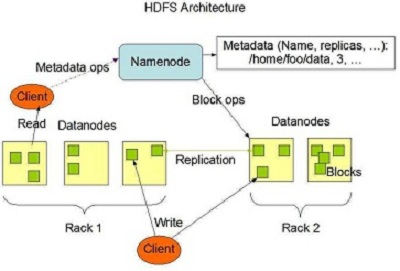
\includegraphics{hdfsfw}
\caption{hdfs框架}
\label{fig:hdfsfw}
\end{figure}

HDFS在本文的设计中起分布式存储的作用,系统中的原始图像库,序列化图像库,特征库以及运行日志都保存在HDFS中。

\section{研究问题及研究现状}
本文研究的重点是如何加速海量图像库的特征提取工作,因为根据之前的分析,特征提取是基于图像内容检索的最为重要技术,并且耗时十分长,因此该研究问题实际意义十分强。

关于图像特征提取问题的研究,很早就有学者开展研究了,而特征提取发展中具有里程碑式的工作应当是Lowe等人在2000年提出的SIFT算法,该算法具有局部不变的特性,意味着在物体被旋转或者是被遮挡的情况下,都不会影响图像的识别,并且算法对光线、噪声、微视角改变的容忍度也相当高。基于这些特性,它们是高度显著而且相对容易撷取,在母数庞大的特征数据库中,很容易辨识物体而且鲜有误认,但是由于该算法的时间复杂性高,特征提取时间难以满足实时要求,后续有许多研究者在SIFT算法的基础上做改进,以提高特征提取的时间。

目前针对SIFT算法性能优化的研究主要集中在两个方面。一是改进算法以降低时间开销、提高特征提取速度。例如Bay提出的SURF(Speeded Up Robust Features)[引用]延续SIFT算法的思想,通过积分图像和Haar小波相结合提高特征提取的速度;Ethan R.等人提出的ORB算法[引用]采用了一种快速的基于Brief的二进制特征描述子方法提高了特征检测速度;Matas等人则提出了最大极值区域(MSERS, Maximally stable Extremal Regions)特征检测方法[引用],借用分水岭的思路检测图像中灰度最稳定的局域区域,然后对检测区域进行旋转和尺度的归一。二是借助FPGA、GPU等硬件加速器提高SIFT算法的性能,例如S.Heyman等人将SIFT算法移植到GPU上[引用],获得了不错的性能加速。本文则研究了基于Spark优化SIFT算法性能的方法。

大数据处理框架Spark自在Apach上开源以来,一直都受到热烈的关注,有许多研究者都使用Spark进行数据的处理,包括现在十分火热的机器学习,深度学习都有在Spark上应用。但是我们发现Spark现在更多的是进行纯文本的分析,直接对图像进行处理的尚未发现,并且Spark里面也没有对图像处理支持的相关库,因此这也促使我们产生在Spark上进行图像处理的相关研究,因此我们就选取了图像处理中的特征提取步骤,在Spark上开展研究。

\section{本文工作与成果}
\begin{figure}[htp]
\centering
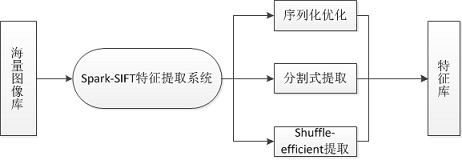
\includegraphics{workfw}
\caption{工作成果展示}
\label{fig:workfw}
\end{figure}
如图~\ref{fig:workfw}所示,针对大规模图像特征提取,我们设计了一个基于Spark大规模图像特征提取系统Spark-SIFT,然后,我们针对该系统提出了三种优化方案。首先,我们针对单个图片体积较少,而HDFS读写小文件效率又不高问题,我们对系统进行了序列化优化。然后,针对Spark现有的任务划分方式造成的负载不均衡问题,我们提出了分割式的特征提取算法。最后,我们针对分割式算法的基础上,进一步优化,提出了Shuffle-efficient 的特征提取算法。具体研究内容概括如下:
\begin{compactenum}
\item 大规模图像库分布式提取系统Spark-SIFT\\本文首先实现了一个Spark下的图像处理基础库SparkImgLib,然后基于SparkImgLib,本文实现了Spark 框架下的SIFT算法。在此基础上设计了一个大规模的图像库特征提取系统。
\item 序列化优化\\HDFS在读写小文件时性能较低,而处理的图片体积一般是比较小的,比如几百K,因此本文设计中设计了一个序列化模块进行图片的预处理,将图片以record的形式保存到HDFS中,提升了读写的性能。
\item 分割式特征提取算法\\Spark在进行任务划分时只考虑了task总体积,但是这种划分方式在本文设计中可能会造成tasks的负载不均衡,因为图片本身大小也会影响tasks的运行时间,针对这一点,我们提成了分割式的图片特征提取算法,将较大的图片分割成子块,来改善Spark在因为tasks划分方式导致的负载不均衡问题。
\item Shuffle-efficient特征提取算法\\Spark中Shuffle机制是影响性能的重要因素。分割式提取算法中存在Shuffle问题,比如同一图片的子块散落在不同的分区时的数据混洗以及在不同分区上收集同一张图片子块时的数据混洗。针对上述Shuffle问题,我们提出了shuffle-efficient的特征提取算法,提升shuffle性能。
\end{compactenum}

\section{论文结构}
本文一共分为6个章节,总体结构如图~\ref{fig:paperfw}所示:
\begin{figure}[htp]
\centering
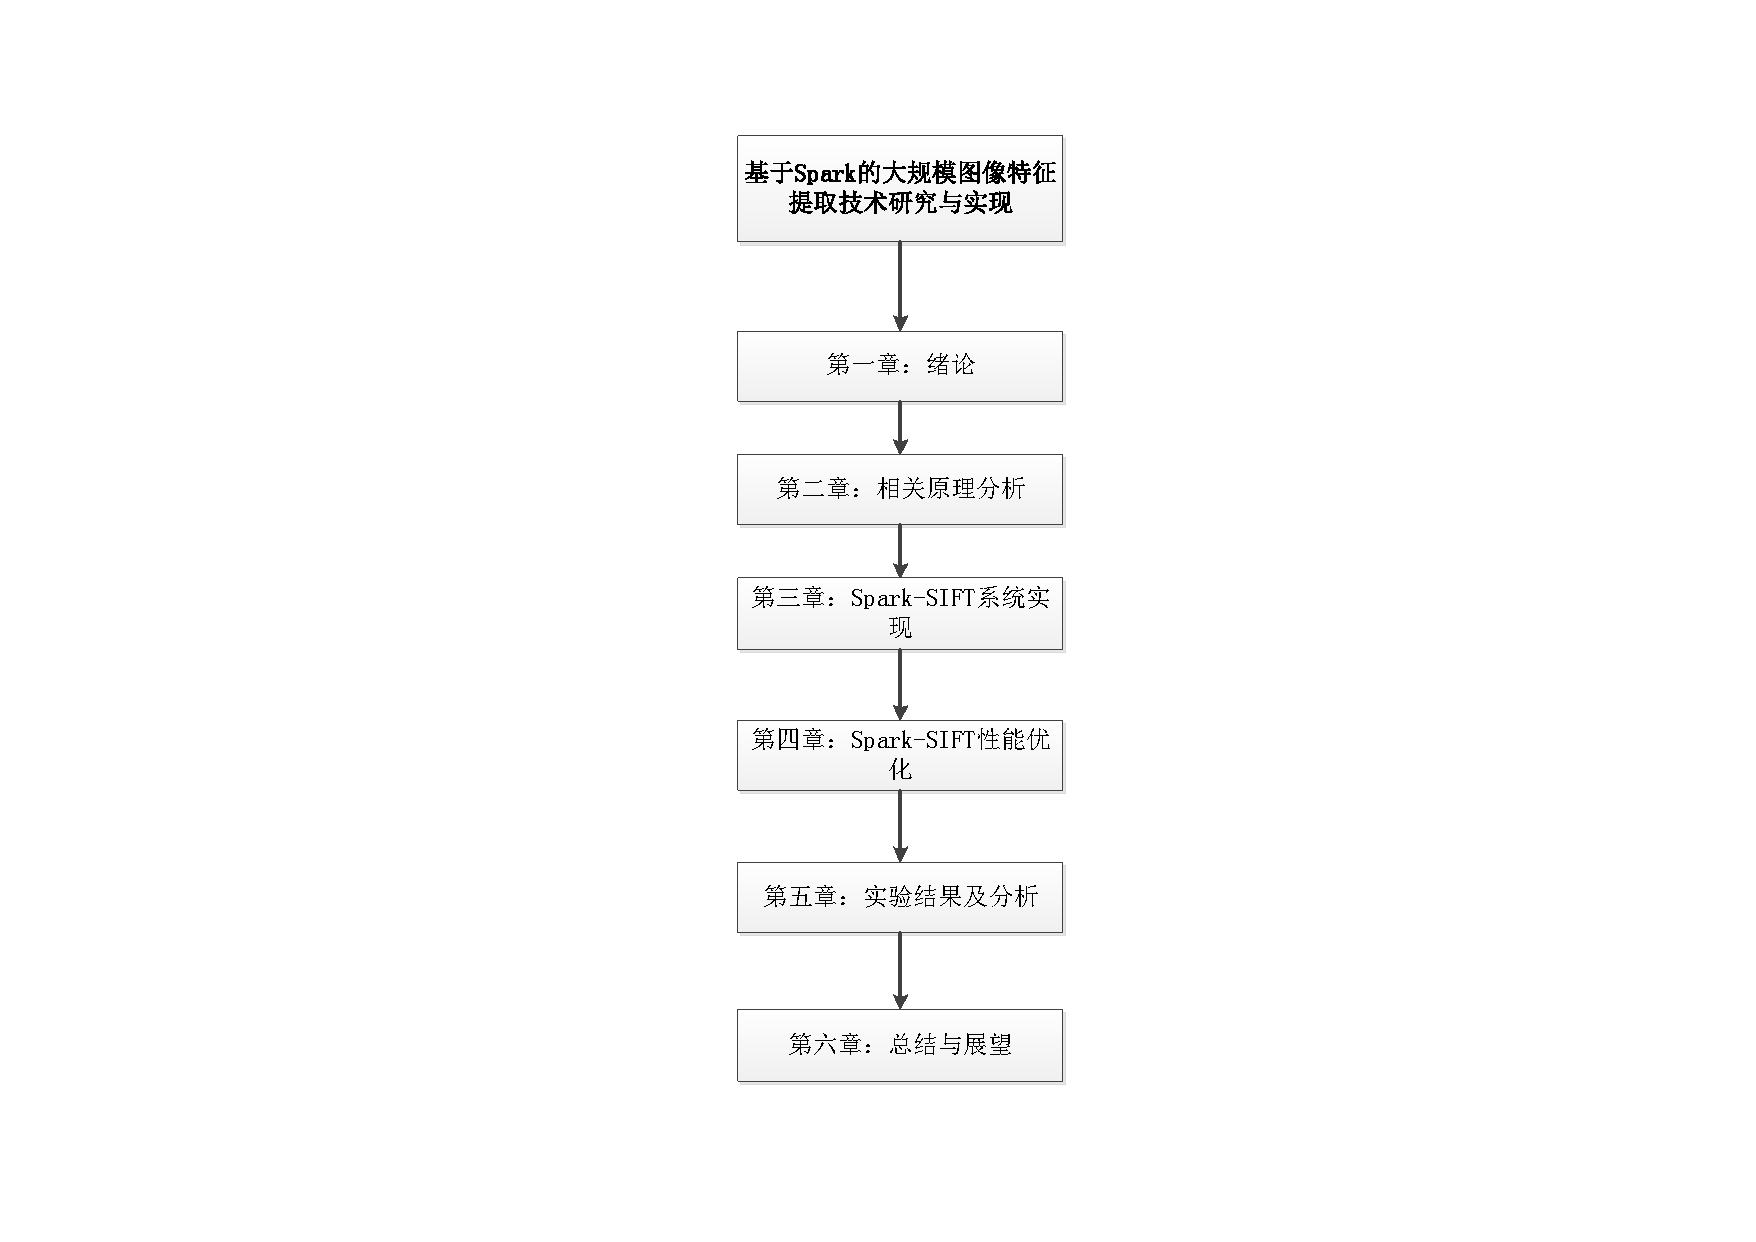
\includegraphics{paperfw}
\caption{论文组织结构}
\label{fig:paperfw}
\end{figure}

第一章为绪论,在绪论中,我们首先讨论了基于文本的图像检索技术和基于内容的图像检索技术的区别,解释了基于内容的图像检索技术存在意义,进而引出了基于内容的图像检索中的两个关键技术,分别是图像特征提取技术和图像匹配技术。对于特征提取部分,我们阐述了图像特征的分类及对应的提取方法。对于特征匹配部分,我们解释了匹配的基本原理及几种度量方式的特点和区别。在介绍完图像关键处理技术后,我们分析了大数据处理技术,在这部分内容中,我们主要介绍了本系统设计中的两个大数据处理框架Spark和HDFS,我们分析了它们的存在的价值,技术特点,及在本文设计中扮演的角色。最后,介绍了本文的研究问题及问题研究现状,本文工作成果以及论文结构三部分。

第二章,本文分析了设计中所涉及的一些原理知识,这些知识为本文的设计工作提供理论基础。

第三章,介绍了大规模图像库特征提取系统Spark-SIFT系统的整体设计工作。

第四章,介绍了在Spark-SIFT基础上提出的三种优化方案,分别是序列化优化,分割式特征提取算法以及shuffle-efficient特征提取算法。

第五章分析了实验结果

第六章总结了本文的所有设计工作及创新点,分析了存在的不足点,最后对未来工作的一些看法和展望。


